\chapter{Diagnóstico}

Neste capítulo são apresentadas as análises realizadas do \textit{framework} CodeIgniter e do PHPUnit e a definição das \textit{features} para o \textit{framework} de testes proposto.

    
\section{Testes no CodeIgniter}

O \textit{framework} CodeIgniter\footnotemark possui uma classe de testes que dispõe de uma função de avaliação
e duas funções de resultado. 
\footnotetext{Informações retiradas do Manual do CodeIgniter. Disponível em \url{http://www.codeigniter.com/user_guide/libraries/unit_testing.html}. Acesso em 22/05/2016.}

Para realizar um teste deve-se executar o comando \textit{\$this->unit->run} passando como parâmetro
o que se deseja testar, o resultado esperado, o nome do teste, e alguma nota (texto) associada, respectivamente.

A classe provê alguns tipos de comparação pré-definidos para serem colocados como o resultado esperado. São eles:

\begin{table*}[!h]
\caption{Tipos de comparação da classe de testes}
\label{table:tipos_comparacao}
\centering
\begin{tabular}{|p{0.25\linewidth}|p{0.25\linewidth}|}
  \hline
  \multicolumn{2}{|c|}{\textbf{Tipos}} \\
  \hline			
	is\_object & is\_string \\
  \hline
	is\_bool &	is\_true \\
  \hline
	is\_false & is\_int \\
  \hline
	is\_numeric & is\_float \\
  \hline
	is\_double & is\_array \\
  \hline
	is\_null &	is\_resource \\
  \hline
  \end{tabular}
\end{table*}

Para obter um relatório completo sobre os testes o comando a ser executado é \textit{\$this->unit->report}, 
o relatório é obtido no formato HTML. Para o resultado completo sem formatação a palavra \textit{report} deve ser
substituida por \textit{result}.

Para cada teste do relatório são apresentados o nome do teste, o tipo de dado do teste, o tipo de 
dado do resultado esperado, o resultado, o nome do arquivo, o número da linha e as notas associadas.
Um exemplo deste relatório pode ser visto na figura \ref{fig:relatorio_codeigniter}.

\begin{figure}[!h]
\centering
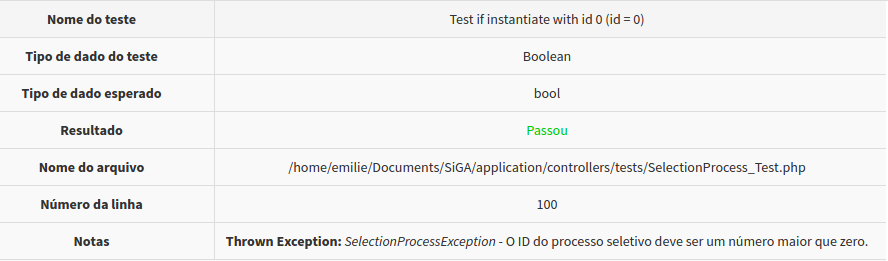
\includegraphics[scale=0.7]{figuras/relatorio_codeigniter.png}
\caption{Relatório de teste do CodeIgniter}
\label{fig:relatorio_codeigniter}
\end{figure}

Na figura \ref{fig:fluxo_codeigniter} é apresentado o fluxo seguido para realização de testes de uma classe no CodeIgniter.

\begin{figure}[!h]
\centering
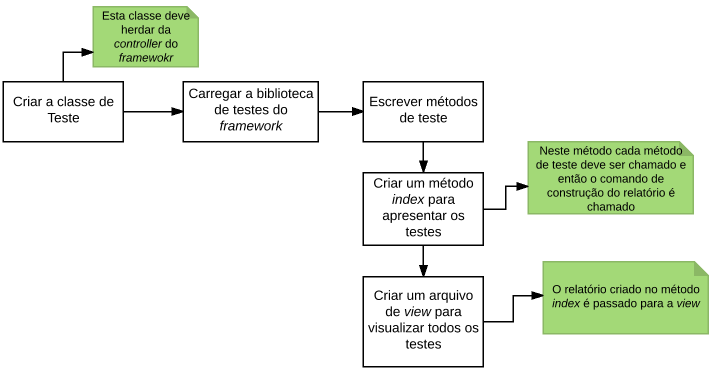
\includegraphics[scale=0.7]{figuras/fluxo_codeigniter.png}
\caption{Fluxo de criação de teste do CodeIgniter}
\label{fig:fluxo_codeigniter}
\end{figure}

Observando o fluxo de criação e execução de testes no CodeIgniter é possível perceber que é uma classe simples que não provê muitos recursos. Além disso a execução dos testes é pouco automatizada, visto que é necessário chamar cada método
de teste escrito. 

\vfill
\pagebreak


\section{O \textit{framework} de testes PHPUnit}

  O PHPUnit\footnotemark  é um \textit{framework} de testes para PHP bastante completo e com suporte adequado
  da comunidade. A versão estável mais atual é a 5.3, podendo ser instalado utilizando o gerenciador
  de dependências \textit{Composer}. As configurações são realizadas por meio de um arquivo XML que é 
  executado antes dos testes.
  \footnotetext{Informações retiradas do Manual do PHPUnit. Disponível em \url{https://phpunit.de/}. Acesso em 22/05/2016.}
  
  Largamente utilizado pela comunidade PHP, o PHPUnit oferece recursos de testes unitários até
  testes funcionais. Como o foco deste trabalho consiste em testes unitários e de integração, serão
  apresentados os recursos do \textit{framework} que possam ser utilizados nesses níveis de teste.
  
  \subsection{Convenções}
    
    O PHPUnit segue algumas convenções, que são apresentadas logo abaixo.
    
    \begin{itemize}
      \item As classes de teste devem ser sufixadas com \textit{'Test'};
      
      \item As classes de teste geralmente herdam da classe base \textit{'PHPUnit\_Framework\_TestCase'};
      
      \item Os testes devem ser métodos públicos prefixados com \textit{'test'}.
    \end{itemize}

  
  \subsection{Recursos gerais}
  
    A seguir são listados alguns recursos gerais do \textit{framework}:
    
    \begin{itemize}
      \item Suporte à anotações \footnotemark ;
	\footnotetext{Apêndice de anotações do PHPUnit. Disponível em \url{https://phpunit.de/manual/current/pt\_br/appendixes.annotations.html}.
		      Acesso em 22/05/2016.}
		      
      \item Completa biblioteca de assertivas com a possibilidade de customização;
	
      \item Declaração explícita de dependência entre testes (dizer que um método teste depende do retorno de outro);
      
      \item Métodos provedores de dados para outros testes;
      
      \item Converter erros e avisos do PHP para exceções tratáveis no teste;
      
      \item Teste de saídas (\textit{'echo'} e \textit{'print'});
	\subitem Útil para testar resultados retornados via ajax.
	
      \item Suporte à linha de comando;
      
      \item \textit{Fixtures};
      
      \item Composição de suíte de testes;
      
      \item Possibilidade de definir o tempo máximo de execução do teste;
      
      \item Possibilidade de marcar testes como incompletos;
      
      \item Extensão \textit{DbUnit} para automatizar testes com banco de dados. Oferece:
	\begin{itemize}
	 \item Toda a estrutura para manter o banco de dados de testes, com funções para conexão
		com o banco, assertivas específicas, definição de \textit{datasets}, preparação
		e destruição do ambiente de teste, entre outros;
	 \item Suporte a diferentes tipos de \textit{datasets}(FlatXML, XML, YAML, CSV).
	\end{itemize}
      
      \item Suporte a \textit{Mocking} com \textit{Stubs};
	\subitem Possibilidade de utilização do \textit{framework} Prophecy \footnotemark para realizar Mock.
	  \footnotetext{\textit{Prophecy Mocking Framework}. Disponível em \url{https://github.com/phpspec/prophecy}. Acesso em 22/05/2016.}
	
      \item Cobertura de código altamente configurável e com métricas;
	 \subitem Relatório de cobertura de código em XML, HTML ou TEXT.
      
      \item \textit{Logging} dos resultados em diferentes formatos configuráveis (XML, TAP, JSON);
      
      \item Alta extensibilidade.
	\subitem É possível criar classes base de teste específicas, o que pode ser bastante útil para utilizar com o CodeIgniter.
    \end{itemize}
    
  \subsection{Problemas encontrados com os recursos disponíveis}
    
    As funcionalidades oferecidas pela extensão \textit{DbUnit} são bastante completas e atenderiam bem às necessidades
    para um teste de integração.
    Entretanto, além do \textit{DbUnit} não subir a mesma estrutura do banco da aplicação para o banco de teste,
    o que tem que ser realizado a parte dos testes, o \textit{DbUnit} oferecido pelo PHPUnit utiliza a abstração PDO para
    criar uma conexão direta com o banco de dados, enquanto a conexão com o banco de dados é encapsulada dentro do CodeIgniter,
    o que impossibilita o uso direto do \textit{DbUnit} no CodeIgniter para realizar os testes de integração que necessitem de
    acesso ao banco de dados.


\section{Possíveis \textit{Features} do \textit{framework}}

\begin{itemize}

	\item Classe base para teste unitário
	\item Classe base para teste de integração \textit{controller-model}
	\item Elaborar esquema de criação de dados no banco de dados (\textit{migration} de teste)
	\item Reconhecimento da \textit{controller} que está sendo testada
		\subitem Ex: CourseTest (Classe de Teste) -> Course (\textit{Controller})
	\item Fazer esquema de subir o banco pro teste e depois limpar o banco
	\item Elaborar uma forma para criar dados fixos para o banco de teste (similar ao Bootstrap do Grails);
	\item Classe base para teste de helper
	\item Classe base para teste de módulo
	\item Classe base de teste funcional
	\item Fazer \textit{mock}

\end{itemize}

\section{\textit{Features} selecionadas}

Como escopo deste trabalho serão implementadas somente as \textit{features}: Classe base para teste unitário
e Classe base para teste de integração \textit{controller-model}.